\begin{figure}[t]
    \centering
    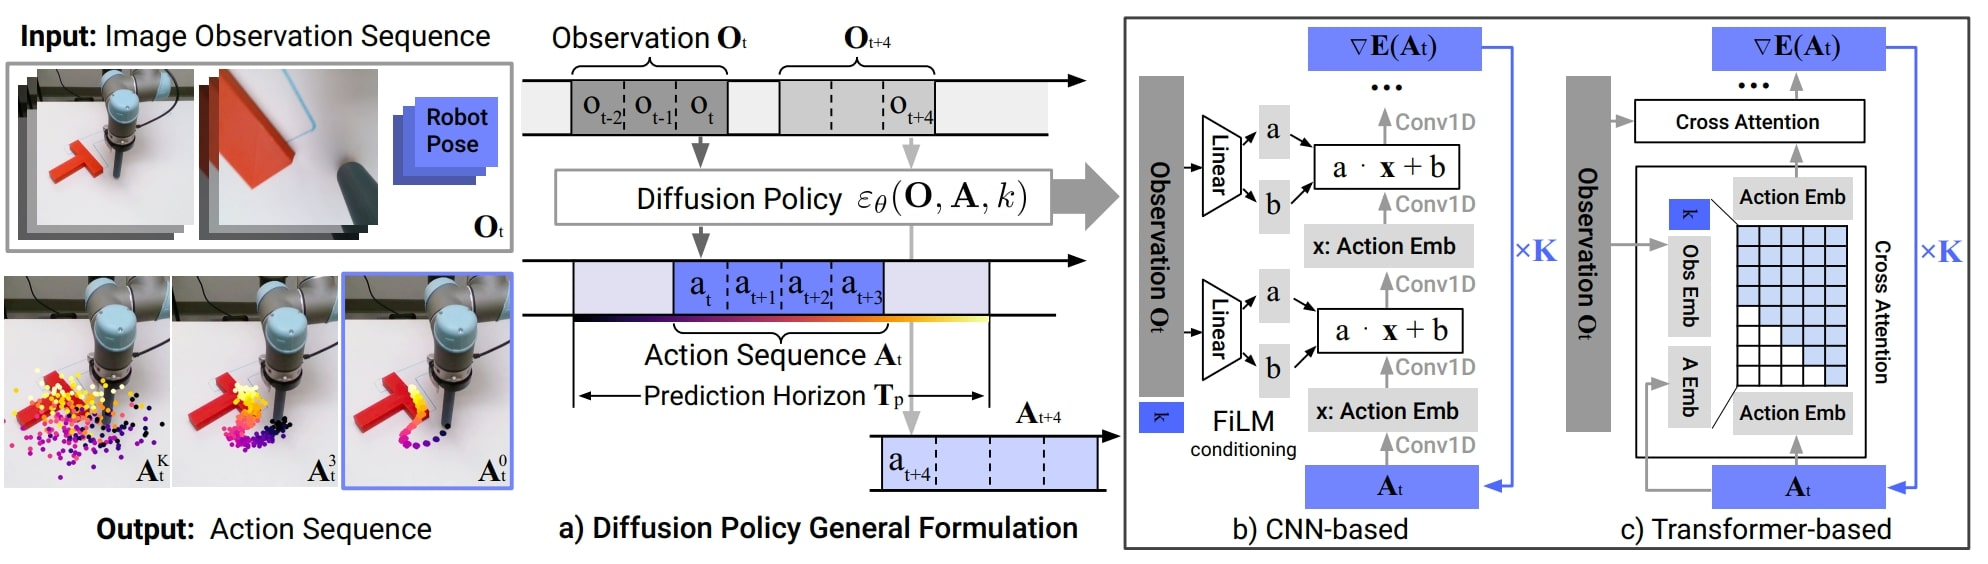
\includegraphics[width=\textwidth]{figures/images/diffusion_policy/diffusion_model.jpg}
    \caption{Architecture presented in \cite{cheng2023diffusion}. (a) General formulation, at time step $t$, the policy inputs the latest $T_o$ steps of observation data $O_t$ and outputs $T_a$ steps of actions $A_t$. (b) CNN-based Diffusion Policy, the observation feature $O_t$ is conditioned using FiLM \cite{perez2018film}. Starting with $A_t^K$ from Gaussian noise, the noise-prediction network $\epsilon_\theta$ iteratively subtracts noise to obtain the denoised action sequence $A_t^0$. (c) Transformer-based Diffusion Policy, the observation embedding $O_t$ is fed into a multi-head cross-attention layer within each decoder block, with causal attention applied to constrain each action embedding to attend only to itself and prior actions.}
    \label{fig:diffusion_model}
\end{figure}
